Hver av signalene på input slås sammen før dem går inn i opampen.
I følgende krets har input forskjellig motstand, men de kan like så godt
ha samme motstand.
Lik motstand kan f.eks. brukes i et miksebord for lyd.
Ulik motstand kan brukes, som i bildet, til å konvertere binær til analog.

\begin{figure}[H]
  \caption{Addisjon med opamp}
  \centering
  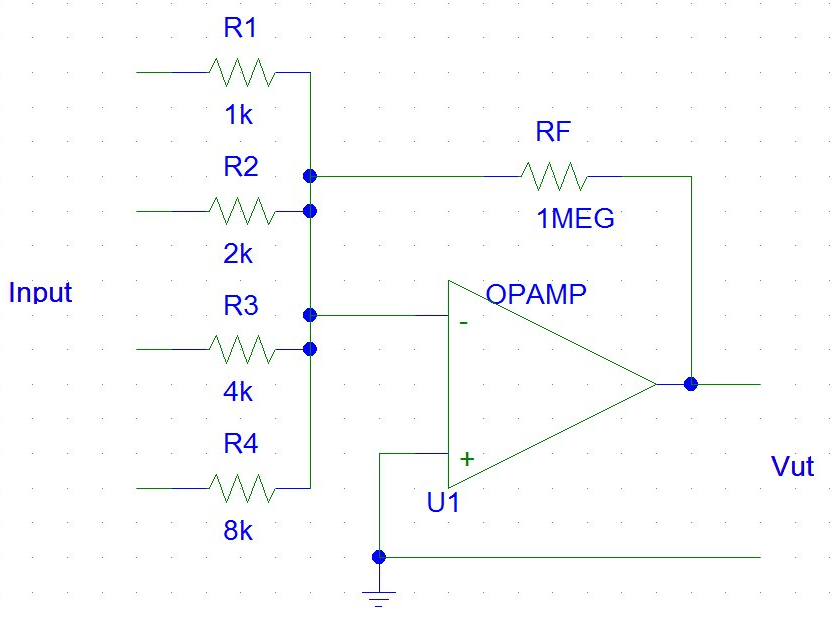
\includegraphics[width=0.67\textwidth]{./img/addisjon.png}
\end{figure}

Strømmen inn i knutepunktet er lik strømmen ut av det.
$$i_1 + i_2 + i_3 + i_4 = i_f + i_i$$
$$v_i \approx = 0 \rightarrow i_i = 0$$
Det gir at
$$\frac{v_1}{R_1} + \frac{v_2}{R_2} + \frac{v_3}{R_3} + \frac{v_4}{R_4}
  = -\frac{v_o}{R_f} \rightarrow v_o
  = -\left( v_1\frac{R_f}{R_1} +...+ v_4\frac{R_f}{R_4} \right)$$

Leddene $\frac{R_f}{R_n}$ kalles vekt og avgjør hvor mye hver av inputene skal
telle med i resultatet.
For et miksebord kan justering av channel gain endre på en slik vekt.
Master volumet kan justeres ved $R_f$.
